\section{Future Work} \label{sec:futureWork}

In our current implementation, we stream the video in SVEF which is using RDP only. However, this is not a good choice in real world. The scenarios we design only suit in experimental environments. Clients may want to receive a video content with lower quality instead of request a high quality video but receive something terrible. Furthermore, if the P4-based switch detect a network congestion. It should be able to send a message to server and reduce the sending rate. In the future, we will design an algorithm to adjust bitrate (sending rate) dynamically.

To implement this, we are going to use a SDN controller. Open Network Operating System(ONOS)~\cite{berde2014onos} is chosen because it is an  opensource project and it can work great with a P4 switch. ONOS is a modern SDN controller that provides some protocol, some applications, some tutorials, etc, and support by Google and Barefoot. There are already many SDN controllers and control protocols are using in the world. The reason we choose ONOS even it is still in development stage is that they design a new protocol for P4, P4Runtime~\cite{P4Runtime}.

As we mention above. There are already many protocols are used, should we design a new one? The condition is, if we design a protocol as we needed. There will just be one more alternative protocol. Therefore, ONOS provides a target independent, protocol independent, and pipeline independent protocol, which is P4Runtime. P4Runtime is a protocol for runtime control P4-defined switch. It provides protobuf-based APIs and automatically generates stubs for many languages. gRPC is a possible RPC transport. Moreover, this protocol won't change the P4 program running in the p4-target. In contrast, The target should provide a driver to tell ONOS how do they implement the pipeline and other architectures. Sometimes we want to use the controller to update P4 program or push new table into match+action table. P4Runtime also support this.

We design a topology to implement in the future. The network we design includes a sender, a controller, one Barefoot switch, three Raspberry Pi switches (with bmv2), and a receiver, as revealed in Fig.~\ref{scenario_3}. ONOS as a SDN controller is in charge of compiling P4 program and deploy to Barefoot switch and other RPis running bmv2. All the P4-target are also running P4Runtime to communicate with ONOS. All the links are Fast Ethernet cables. The bandwidths of links $d$ and $e$ are higher than the bandwidths of links $f$ and $g$. We physically remove link $e$ during streaming, and we expect to see that the ONOS controller reroutes the video stream through the Raspberry Pi 3 at the bottom. Because we configure links  $f$ and $g$ to have lower bandwidth, the video quality goes down. When we plug the Ethernet cable back, the ONOS controller reroutes the video stream over the Barefoot switch, and the quality of video stream goes up. 

\begin{figure}[tbh]
	\centering
	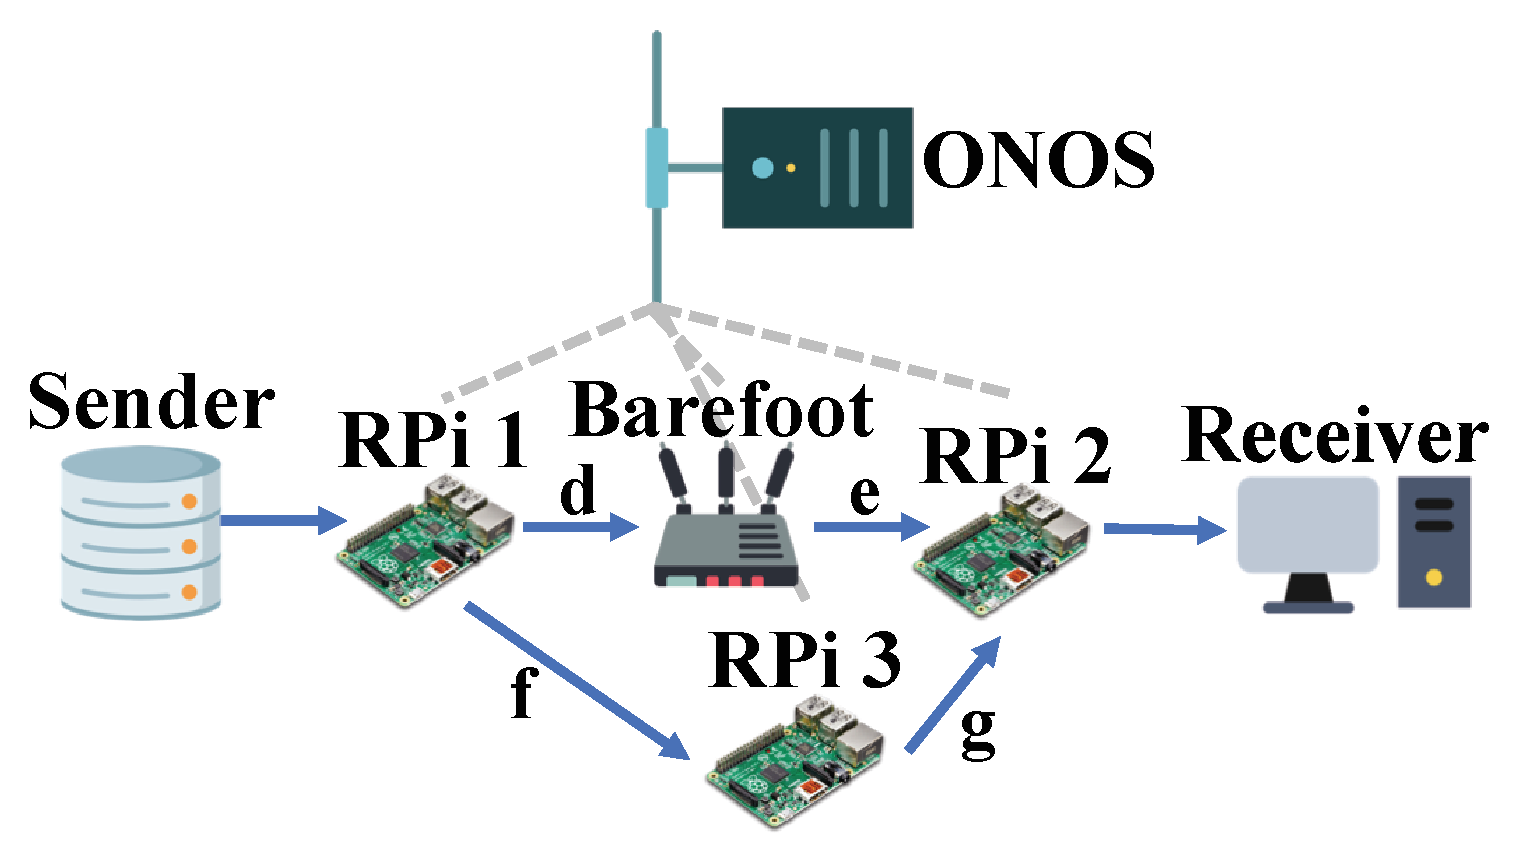
\includegraphics[width=.30\textwidth]{fig/scenario_3.eps}
	\caption{Future work Topology.}
	\label{scenario_3} 
\end{figure}